\documentclass[11pt,a4paper]{scrarticle}
\usepackage[utf8]{inputenc}
\usepackage{cmap}
\usepackage[T2A]{fontenc}
\usepackage[russian]{babel}
\usepackage{amsmath,amssymb,amsthm,mathtools}
\usepackage{array}

\usepackage{indentfirst}
\usepackage{xcolor,graphicx, tikz, wrapfig}
\usepackage{longtable}
\usepackage{nicematrix}

\usepackage{minted}
\usemintedstyle{vs}

\usepackage[left=2cm,right=2cm,top=2cm,bottom=2cm,bindingoffset=0cm]{geometry}

\usepackage[unicode]{hyperref}
\definecolor{linkcolor}{HTML}{0000E6}
\definecolor{urlcolor}{HTML}{0000E6}
\definecolor{citecolor}{HTML}{0000E6}
\hypersetup{pdfpagemode=None,linktoc=page,citecolor=citecolor,linkcolor=linkcolor,urlcolor=urlcolor,colorlinks=true}

\theoremstyle{definition}
\newtheorem{subtask}{Пункт}

\DeclareMathOperator*{\argmax}{arg\,max}
\DeclareMathOperator*{\argmin}{arg\,min}

\setlength{\parindent}{1cm}

\author{Клычков Максим Дмитриевич}

\begin{document}

\centerline{\textbf{\huge Алгоритмы и структуры данных-1}}
\centerline{\textbf{SET 1. Задача A4.}}
\begin{flushright}
	\emph{Осень 2024. Клычков М. Д.}
\end{flushright}

\begin{figure}[htp]
	\centering
	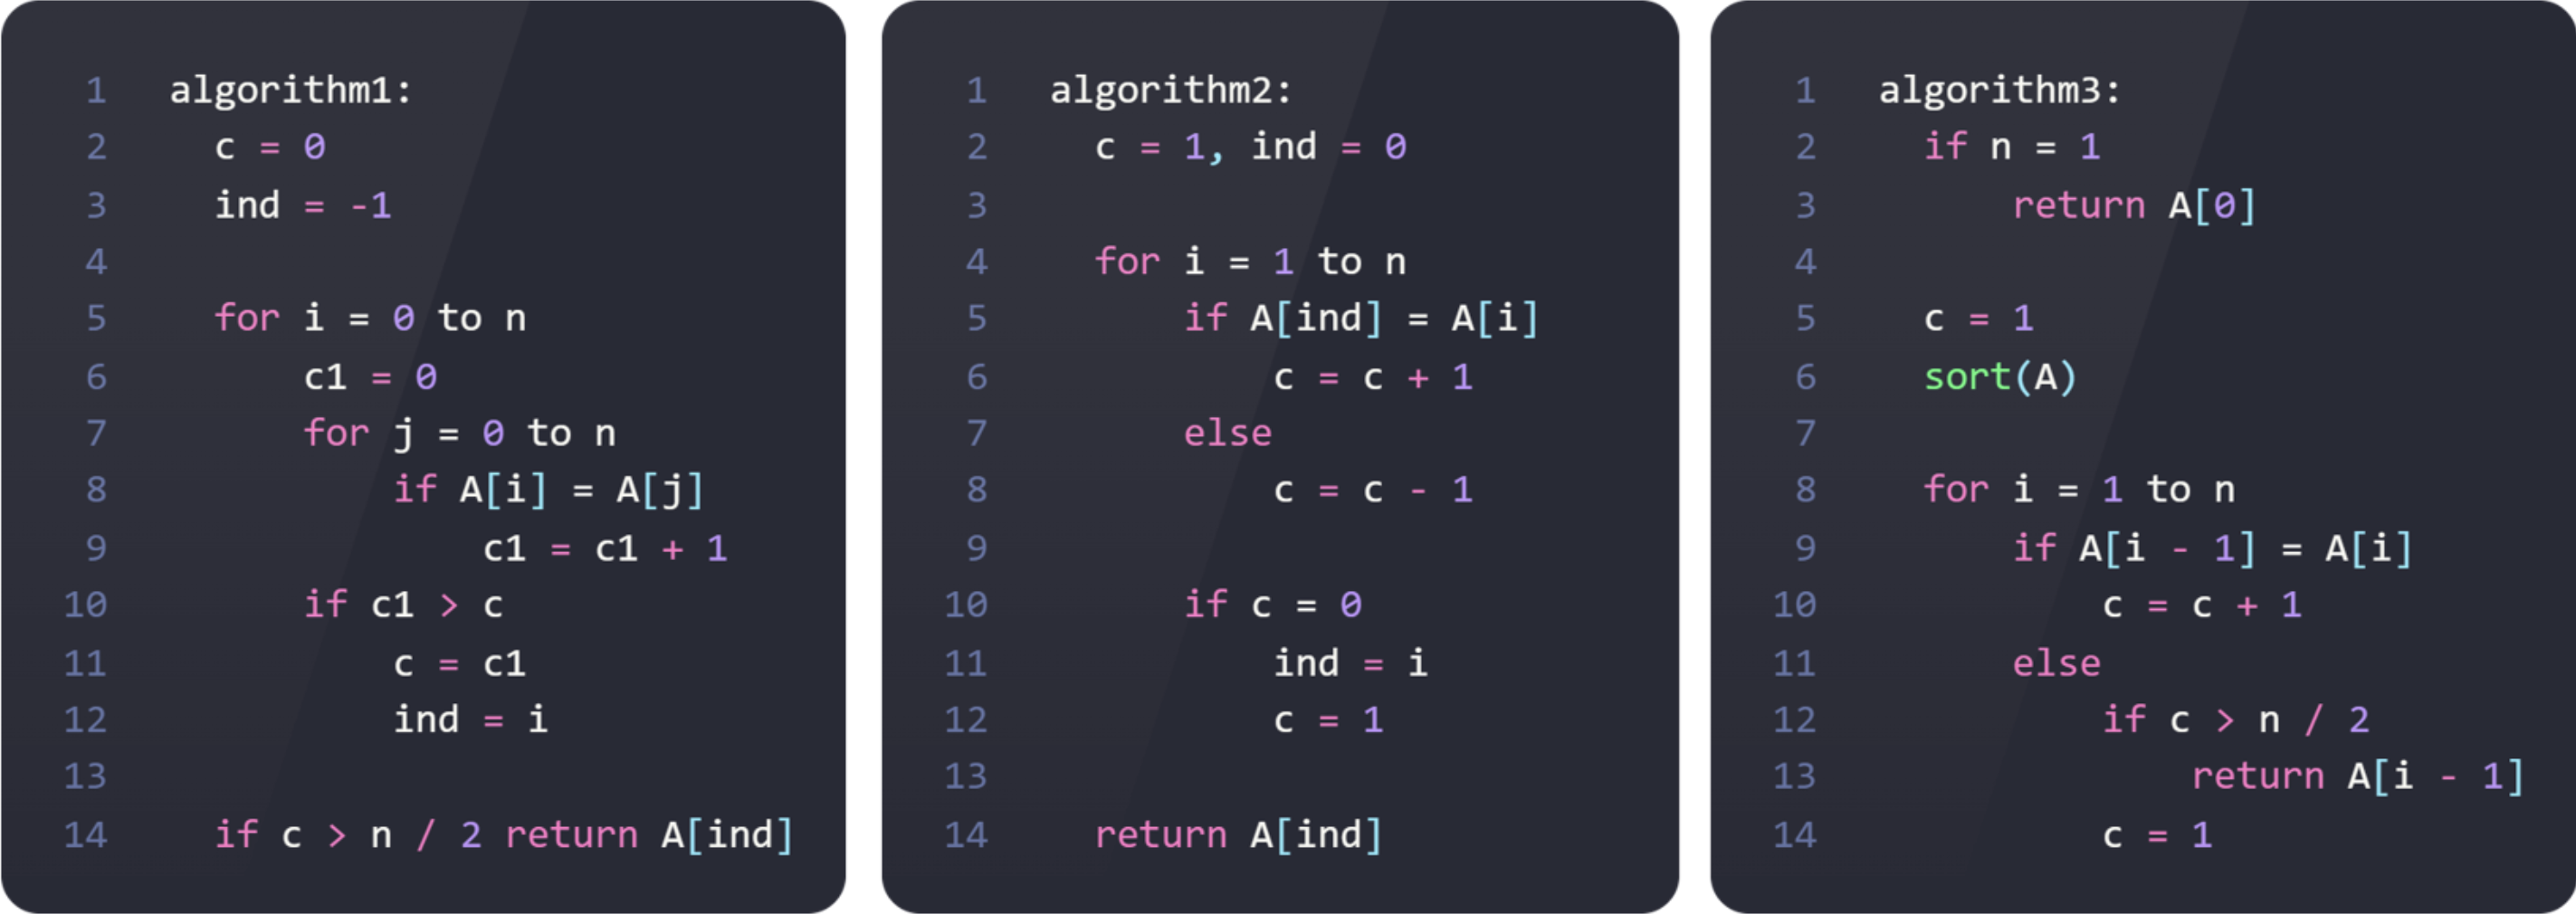
\includegraphics[width=\textwidth]{code.png}
\end{figure}

\begin{subtask}
	Кратко поясним, что делает каждый из приведенных алгоритмов:
	\begin{itemize}
		\item \texttt{algorithm1:} Результат работы алгоритма --- элемент массива, который встречается больше, чем $\left\lfloor \frac{n}{2} \right\rfloor$ раз. Из приведенного псевдокода нельзя сделать вывод о том, что будем выведено, если такого элемента нет.
		\item \texttt{algorithm2:} Тяжело описать, что это «чудо» делает и к какому результату приведет\dots\linebreak Фиксируется элемент (изначально это $A_0$), затем подсчитывается таких же элементов, причем, если встречается отличающийся элемент, то счетчик уменьшается на $1$. Это можно представить графиком (по оси $x$ --- количество обработанных на данный момент элементов, $y$ --- значение счетчика) (рис. \ref{fig:graph}).
		      \begin{figure}[htp]
			      \centering
			      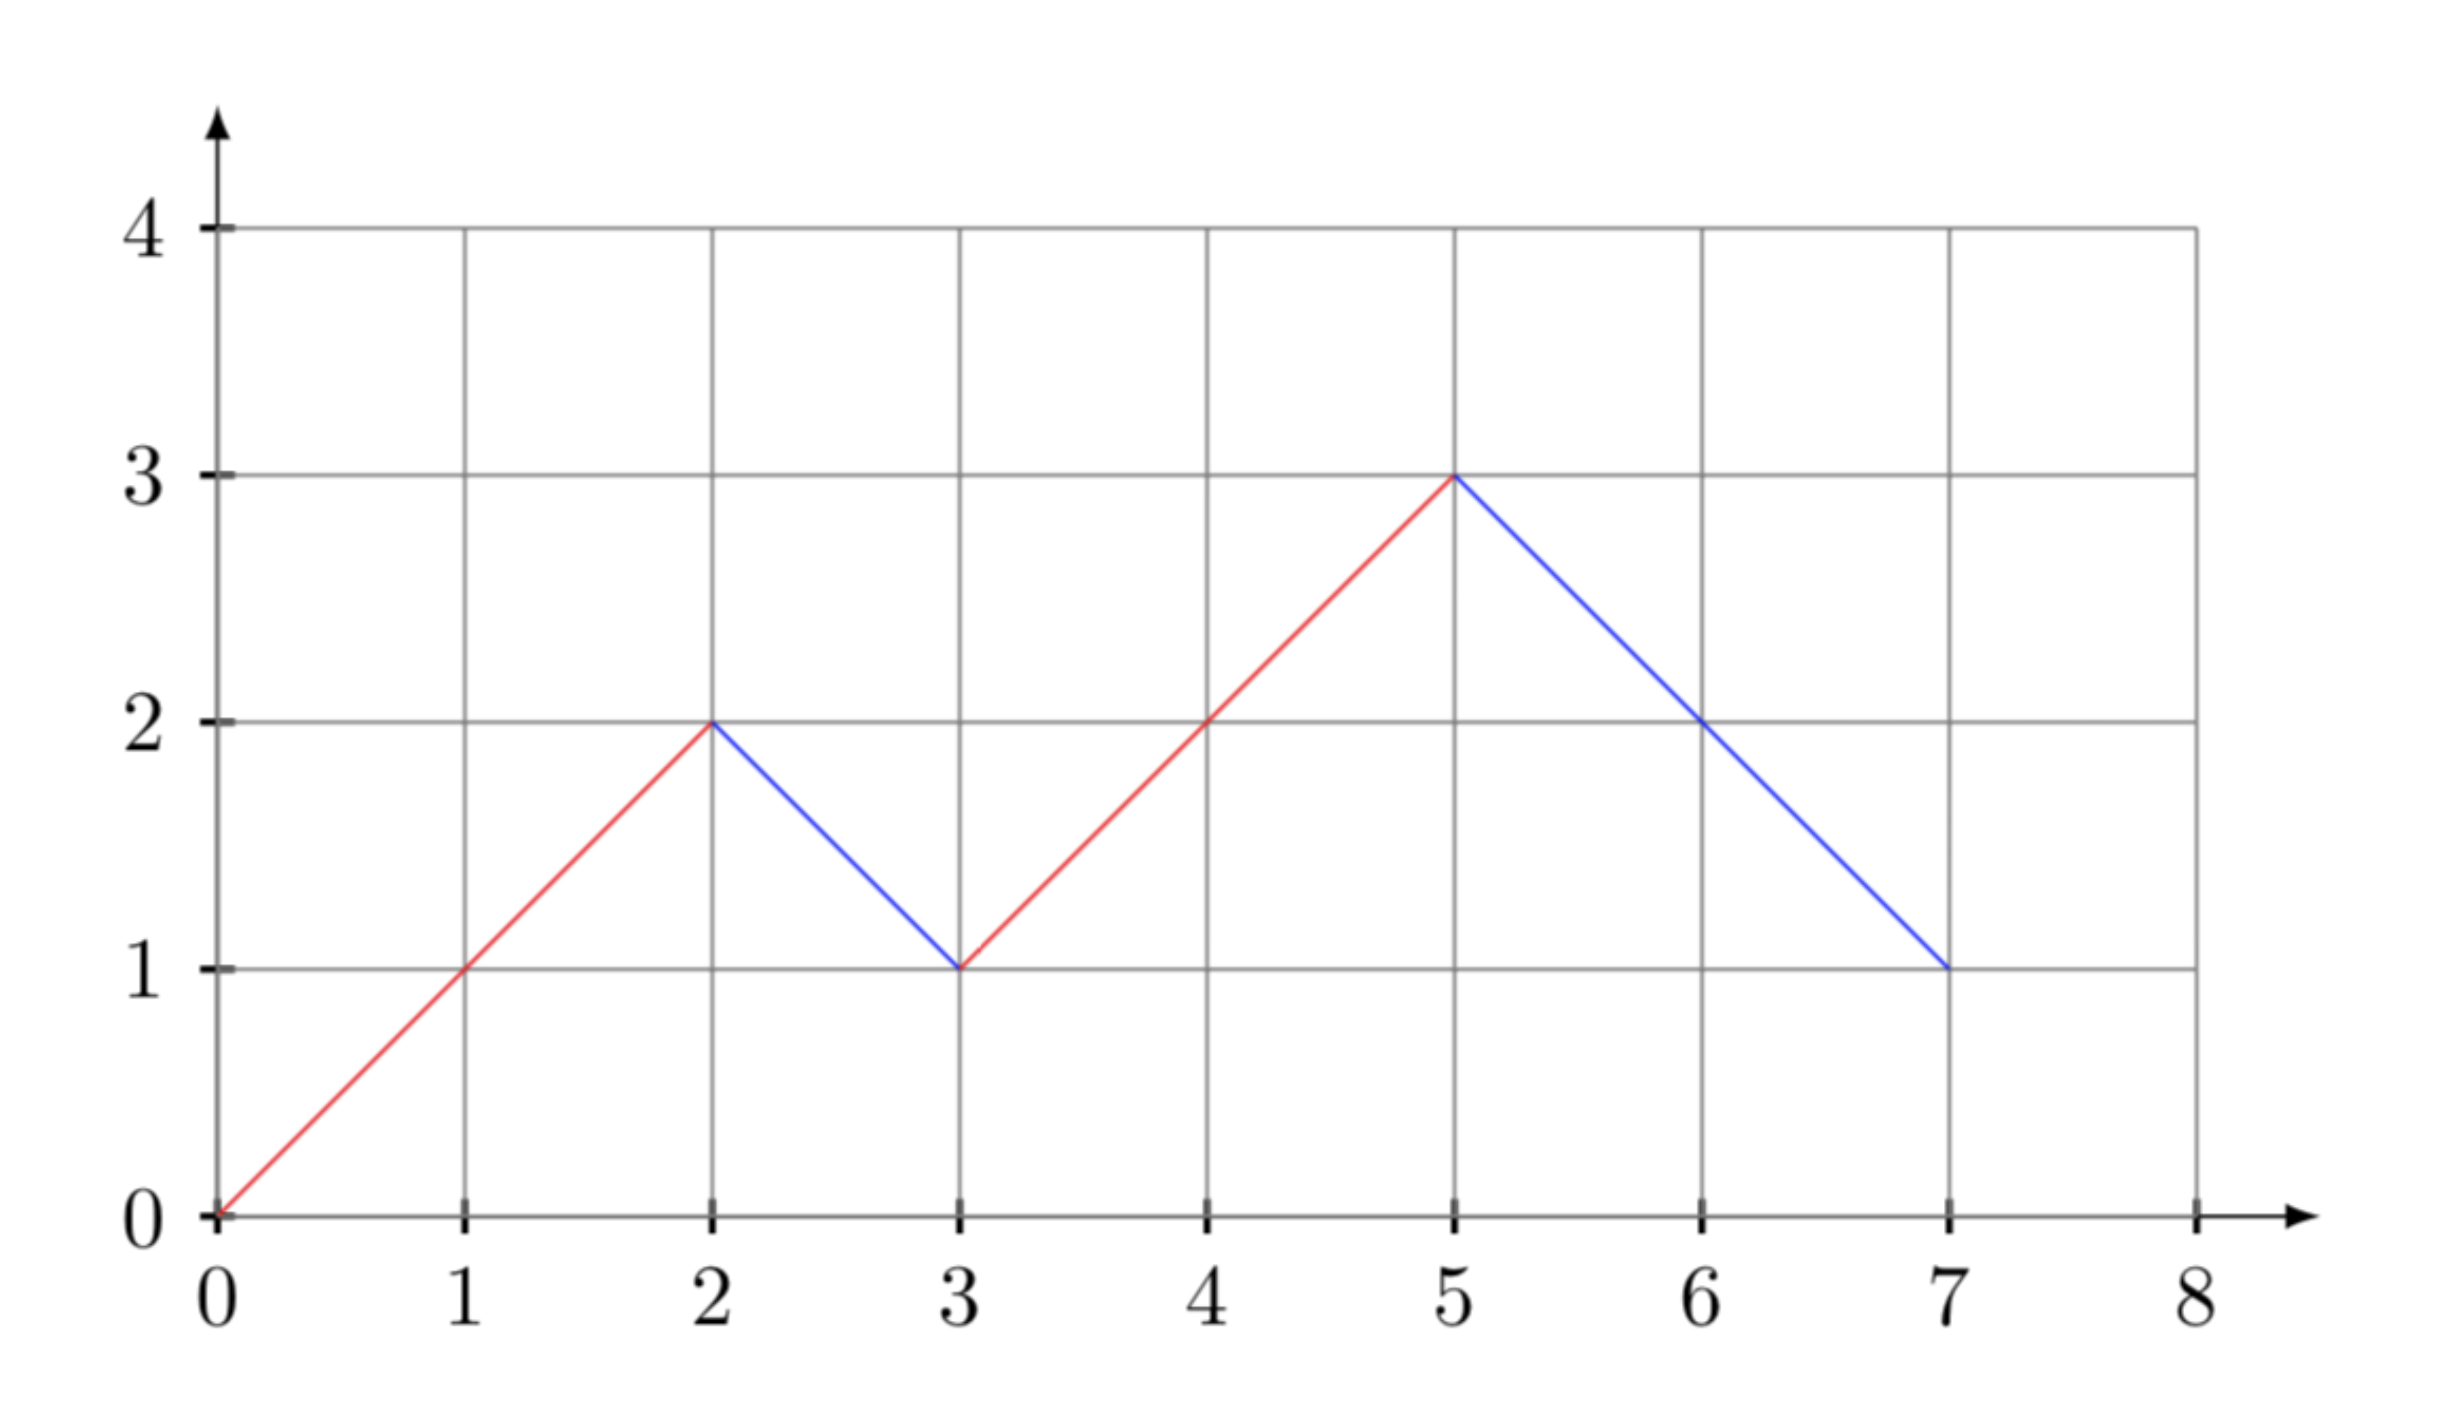
\includegraphics[width=0.6\textwidth]{pic.png}
			      \caption{Графическая интерпретация}
			      \label{fig:graph}
		      \end{figure}

		      После того как линия на графике достигает нуля, счетчик обнуляется и связывается с новым элементом массива. Возвращается элемент, с которым в последний раз был связан счетчик.
		\item \texttt{algorithm3:} Этот алгоритм делает то же самое, что и \texttt{algorithm1}, однако не возвращает результат в том случае, если искомый элемент максимальный (стоит в конце отсортированного массива).
	\end{itemize}

	Можно предположить, что требуется найти элемент, который повторяется больше $n/2$ раз, но никакой из них не реализован корректно, везде есть свои недостатки.

	Приведем примеры:
	\begin{enumerate}
		\item \emph{Результаты работы алгоритмов совпадают.} Пусть $A = \{1, 2, 1, 3, 1, 1\}$. Ожидаем результат: $1$.

		      Приведем частичную трассировку для каждого из алгоритма:

		      \begin{minipage}[t][][c]{0.3\textwidth}
			      \texttt{algorithm1:}
			      \centering

			      \begin{tabular}{|>{$}c<{$}|>{$}c<{$}|>{$}c<{$}|>{$}c<{$}|>{$}c<{$}|}
				      \hline
				      c     & ind   & i     & c_1   & j     \\ \hline
				      0     & -1    &       &       &       \\ \hline
				      0     & -1    & 0     & 1     & 0     \\ \hline
				      0     & -1    & 0     & 1     & 1     \\ \hline
				      \dots & \dots & \dots & \dots & \dots \\ \hline
				      4     & 0     & 0     & 4     & 6     \\ \hline
				      4     & 0     & 1     & 0     & 0     \\ \hline
				      \dots & \dots & \dots & \dots & \dots \\ \hline
				      4     & 0     & 1     & 1     & 6     \\ \hline
				      \dots & \dots & \dots & \dots & \dots \\ \hline
				      4     & 0     & 5     & 4     & 6     \\ \hline
				      4     & 0     & 6     &       &       \\ \hline
			      \end{tabular} \end{minipage}
		      \begin{minipage}[t][][c]{0.3\textwidth}
			      \texttt{algorithm2:}
			      \centering

			      \begin{tabular}{|>{$}c<{$}|>{$}c<{$}|>{$}c<{$}|}
				      \hline
				      c & ind & i \\ \hline
				      1 & 0   &   \\ \hline
				      1 & 1   & 1 \\ \hline
				      1 & 2   & 2 \\ \hline
				      1 & 3   & 3 \\ \hline
				      1 & 4   & 4 \\ \hline
				      2 & 4   & 5 \\ \hline
				      2 & 4   & 6 \\ \hline
			      \end{tabular}
		      \end{minipage}
		      \begin{minipage}[t][][c]{0.3\textwidth}
			      \texttt{algorithm3:}
			      \centering

			      \begin{tabular}{|>{$}c<{$}|>{$}c<{$}|}
				      \hline
				      c & i \\ \hline
				      1 &   \\ \hline
				      2 & 1 \\ \hline
				      3 & 2 \\ \hline
				      4 & 3 \\ \hline
			      \end{tabular}
		      \end{minipage}

		      Действительно, результат работы каждого алгоритма --- $1$.

		\item \emph{Результаты работы алгоритмов отличаются.} Пусть $A = \{1, 3\}$. По сути, должен вернуться «нулевой» результат, так как искомого элемента в массиве нет.

		      \begin{minipage}[t][][c]{0.3\textwidth}
			      \texttt{algorithm1:}
			      \centering

			      \begin{tabular}{|>{$}c<{$}|>{$}c<{$}|>{$}c<{$}|>{$}c<{$}|>{$}c<{$}|}
				      \hline
				      c & ind & i & c_1 & j \\ \hline
				      0 & -1  &   &     &   \\ \hline
				      0 & -1  & 0 & 1   & 0 \\ \hline
				      0 & -1  & 0 & 1   & 1 \\ \hline
				      1 & 0   & 0 & 1   & 2 \\ \hline
				      1 & 0   & 1 & 0   & 0 \\ \hline
				      1 & 0   & 1 & 1   & 1 \\ \hline
				      1 & 0   & 1 & 1   & 2 \\ \hline
				      1 & 0   & 2 &     &   \\ \hline
			      \end{tabular}

			      \texttt{return} не сработает
		      \end{minipage}
		      \begin{minipage}[t][][c]{0.3\textwidth}
			      \texttt{algorithm2:}
			      \centering

			      \begin{tabular}{|>{$}c<{$}|>{$}c<{$}|>{$}c<{$}|}
				      \hline
				      c & ind & i \\ \hline
				      1 & 0   &   \\ \hline
				      1 & 1   & 1 \\ \hline
				      1 & 1   & 2 \\ \hline
			      \end{tabular}

			      Вернется $3$ --- некорректный ответ
		      \end{minipage}
		      \begin{minipage}[t][][c]{0.3\textwidth}
			      \texttt{algorithm3:}
			      \centering

			      \begin{tabular}{|>{$}c<{$}|>{$}c<{$}|}
				      \hline
				      c & i \\ \hline
				      1 &   \\ \hline
				      1 & 1 \\ \hline
				      1 & 2 \\ \hline
			      \end{tabular}

			      \texttt{return} не сработает
		      \end{minipage}
	\end{enumerate}
\end{subtask}

\begin{subtask}
	Пусть $T_1(n)$, $T_2(n)$, $T_3(n)$ --- функции временной сложности для алгоритмов \linebreak \texttt{algorithm1}, \texttt{algorithm2} и \texttt{algorithm3} соответственно.

	Оценим приблизительно эти функции.

	\begin{enumerate}
		\item В \texttt{algorithm1} используется двойной цикл (вложенный), каждый из которых проходит от $0$ до $n$, следовательно, $T_1(n) = O(n^{2})$.
		\item В \texttt{algorithm2} используется один цикл от $1$ до $n$, следовательно, $T_2(n) = O(n)$.
		\item В \texttt{algorithm2} используется сортировка и один цикл от $1$ до $n$. Будем считать, что используется одна из сортировок, работающих за $O(n \log n)$. Тогда, $T_3(n) = O(n \log n) + O(n) = O(n \log n)$.
	\end{enumerate}
\end{subtask}

\begin{subtask}
	Конечно, можно придираться к тому, что некоторые функции не возвращают значения, но будем считать, что там просто возвращается \texttt{Null}, прямо как на языке \texttt{Python}.

	\begin{enumerate}
		\item В алгоритме \texttt{algorithm2} можно определенно не хватает существенной части. После выполненного цикла нельзя утверждать, что элемент $A_{ind}$ является искомым, можно лишь считать, что либо результат не определен (\texttt{Null} подобно \texttt{algorithm1}), либо это действительно верный ответ. Другими словами, элемент $A_{ind}$ --- единственный претендент на ответ. Оставшуюся проверку можно провести вновь за линейное время, например, так:

		      \begin{figure}[h]
			      \centering
			      \begin{minipage}{0.4\textwidth}
				      \begin{minted}{cpp}
cur = 0
for i = 0 to n
  if A[i] = A[ind]
	cur = cur + 1
if cur > n / 2
  return cur
					  \end{minted}

			      \end{minipage}
			      \caption{\texttt{algorithm2} improve}
		      \end{figure}

		      Тогда, чтобы получить работающий код, нужно убрать 14 строчку и добавить вышеуказанную проверку.
		\item В алгоритме \texttt{algorithm3} нужно дописать следующие строки в конце приведенного, чтобы обрабатывать те повторяющиеся элементы, которые стоят в хвосте отсортированного массива.

		      \begin{figure}[h]
			      \centering
			      \begin{minipage}{0.4\textwidth}
				      \begin{minted}{cpp}
if c > n / 2
  return A[n - 1]
					  \end{minted}

			      \end{minipage}
			      \caption{\texttt{algorithm3} improve}
		      \end{figure}

	\end{enumerate}
\end{subtask}

\begin{subtask}
	Так как в \texttt{algorithm1} никакие улучшения не предлагались, оценим только функции временной сложности улучшенных алгоритмов \texttt{algorithm2} и \texttt{algorithm3}: $T_2'(n)$ и $T_3'(n)$ соответственно.

	$$
		T_2'(n) = T_2(n) + O(n) = O(n) + O(n) = O(n)
	$$

	$$
		T_3'(n) = T_3(n) + O(1) = O(n \log n) + O(1) = O(n \log n)
	$$
\end{subtask}

\end{document}